% Copyright (c) 2023-2025
% This file is part of sep3cs.
%
% sep3cs is free software: you can redistribute it and/or modify
% it under the terms of the GNU General Public License as published by
% the Free Software Foundation, either version 3 of the License, or
% (at your option) any later version.
%
% sep3cs is distributed in the hope that it will be useful,
% but WITHOUT ANY WARRANTY; without even the implied warranty of
% MERCHANTABILITY or FITNESS FOR A PARTICULAR PURPOSE.  See the
% GNU General Public License for more details.
%
% You should have received a copy of the GNU General Public License
% along with sep3cs. If not, see <http://www.gnu.org/licenses/>.
%
\documentclass[spanish]{article}
\usepackage{babel}
\usepackage{float}
\usepackage[T1]{fontenc}
\usepackage[margin=0.5in]{geometry}
\usepackage{graphicx}
\usepackage{indentfirst}
\usepackage[utf8]{inputenc}
% Copyright (c) 2023-2025
% This file is part of sep3cs.
%
% sep3cs is free software: you can redistribute it and/or modify
% it under the terms of the GNU General Public License as published by
% the Free Software Foundation, either version 3 of the License, or
% (at your option) any later version.
%
% sep3cs is distributed in the hope that it will be useful,
% but WITHOUT ANY WARRANTY; without even the implied warranty of
% MERCHANTABILITY or FITNESS FOR A PARTICULAR PURPOSE.  See the
% GNU General Public License for more details.
%
% You should have received a copy of the GNU General Public License
% along with sep3cs. If not, see <http://www.gnu.org/licenses/>.
%
\usepackage{color}
\usepackage{listings}

\lstloadlanguages{C,C++,csh,Java}

\definecolor{blue}{rgb}{0,0,0.6}
\definecolor{cyan}{rgb}{0.0,0.6,0.6}
\definecolor{green}{rgb}{0,0.8,0}
\definecolor{red}{rgb}{0.6,0,0}

\lstset{
  language=csh,
  basicstyle=\footnotesize\ttfamily,
  numbers=left,
  numberstyle=\tiny,
  numbersep=5pt,
  tabsize=2,
  extendedchars=true,
  breaklines=true,
  stringstyle=\color{blue}\ttfamily,
  showspaces=false,
  showtabs=false,
  xleftmargin=17pt,
  framexleftmargin=17pt,
  framexrightmargin=5pt,
  framexbottommargin=4pt,
  commentstyle=\color{green},
  morecomment=[l]{//}, %use comment-line-style!
  morecomment=[s]{/*}{*/}, %for multiline comments
  showstringspaces=false,
  morekeywords={ abstract, event, new, struct,
  as, explicit, null, switch,
  base, extern, object, this,
  bool, false, operator, throw,
  break, finally, out, true,
  byte, fixed, override, try,
  case, float, params, typeof,
  catch, for, private, uint,
  char, foreach, protected, ulong,
  checked, get, set, goto, public, unchecked,
  class, if, readonly, unsafe,
  const, implicit, ref, ushort,
  continue, in, return, using,
  decimal, int, sbyte, virtual,
  default, interface, sealed, volatile,
  delegate, internal, short, void,
  do, is, sizeof, while,
  double, lock, stackalloc,
  else, long, static,
  enum, namespace, string},
  keywordstyle=\color{cyan},
  identifierstyle=\color{red},
}


\geometry{margin=1.2in}

\title{
  Ingeniería de Software \\
  Seminario Integrador \\
}

\author{
  Amanda Noris Hern\'andez \\
  Juan Miguel P\'erez Mart\'inez \\
  Marcos Antonio P\'erez Lorenzo \\
  Maykol Luis Martínez Rodr\'iguez \\
}

\begin{document}
  \maketitle
  \pagebreak
  \tableofcontents
  \pagebreak
  \section{Requerimientos}

\subsection{Requerimientos Funcionales}

Entre las funcionalidades que debe realizar nuestra aplicación web según los deseos del cliente se encuentran:

\begin{enumerate}
  \item[\(\cdot\)] El sistema debe ser capaz de recopilar datos de los jugadores, incluyendo su código, apodo, nivel, clan al que pertenece, cantidad de trofeos, victorias totales, cartas encontradas, máximo de trofeos alcanzados y carta favorita actual.
  \item[\(\cdot\)] El sistema debe ser capaz de recopilar datos sobre las cartas, incluyendo su nombre, descripción, costo de elixir, calidad y tipo.
  \item[\(\cdot\)] El sistema debe ser capaz de recopilar datos sobre las batallas, incluyendo su duración y el ganador.
  \item[\(\cdot\)] El sistema debe ser capaz de recopilar datos sobre los desafíos, incluyendo su nombre, descripción, costo, cantidad de premios que ofrece, fecha en que comienza, tiempo de duración, nivel mínimo necesario para participar y cantidad de derrotas que admite.
  \item[\(\cdot\)] Recopilación de datos sobre clanes, incluyendo su nombre, posición y líder.
  \item[\(\cdot\)] El sistema debe ser capaz de recopilar datos sobre las guerras de clanes, incluyendo su identificador y la fecha de comienzo.
  \item[\(\cdot\)] El sistema debe ser capaz de realizar las consultas especificadas en el proyecto. 
\end{enumerate}

\subsection{Requerimientos no funcionales}

Nuestra aplicación posee como requerimientos no funcionales los siguientes:

\begin{enumerate}
  \item[\(\cdot\)] Usabilidad: El sistema debe ser intuitivo y fácil de usar para los jugadores, independientemente de su nivel de experiencia con este tipo de aplicaciones.
  \item[\(\cdot\)] Seguridad:
    \begin{enumerate}
      \item[\(\cdot\)] Confidencialidad: La información del jugador debe estar protegida y solo ser accesible por el propio jugador y los administradores del sistema.
      \item[\(\cdot\)] Integridad: La información del juego (como las estadísticas de las cartas y los resultados de las batallas) debe estar protegida contra la corrupción y mantenerse consistente.
      \item[\(\cdot\)] Disponibilidad: Los jugadores deben tener acceso garantizado a la información del juego en cualquier momento.
    \end{enumerate}
  \item[\(\cdot\)] Diseño e implementación:
    \begin{enumerate}
      \item[\(\cdot\)] El sistema será implementado en C\#, siguiendo las mejores prácticas de diseño y arquitectura de software.
      \item[\(\cdot\)] Se utilizará una arquitectura en capas (n-layered) para separar las responsabilidades del sistema y facilitar su mantenimiento y escalabilidad.
      \item[\(\cdot\)] Se utilizará Entity Framework como ORM para facilitar el acceso y manipulación de la base de datos.
    \end{enumerate}
  \item[\(\cdot\)] Rendimiento: El sistema debe ser capaz de manejar un gran volumen de datos y proporcionar respuestas rápidas a las consultas.
\end{enumerate}

\subsection{Requerimientos de entorno}

Para el correcto uso de nuestra aplicación, los usuarios deben adherirse a los siguientes requerimientos de entorno:

\begin{enumerate}
  \item[\(\cdot\)] Hardware: El usuario necesitará un dispositivo con conexión a Internet y capacidad para ejecutar un navegador web moderno (como un PC con Windows/Linux, un Mac o un dispositivo móvil).
  \item[\(\cdot\)] Software: El usuario necesitará un navegador web moderno (como Google Chrome, Mozilla Firefox, Safari, etc.) para acceder a la aplicación. No se requiere ninguna instalación adicional ya que la aplicación se ejecuta en el servidor y se accede a través del navegador.
\end{enumerate}

  % Copyright (c) 2023-2025
% This file is part of sep3cs.
%
% sep3cs is free software: you can redistribute it and/or modify
% it under the terms of the GNU General Public License as published by
% the Free Software Foundation, either version 3 of the License, or
% (at your option) any later version.
%
% sep3cs is distributed in the hope that it will be useful,
% but WITHOUT ANY WARRANTY; without even the implied warranty of
% MERCHANTABILITY or FITNESS FOR A PARTICULAR PURPOSE.  See the
% GNU General Public License for more details.
%
% You should have received a copy of the GNU General Public License
% along with sep3cs. If not, see <http://www.gnu.org/licenses/>.
%
\section{Funcionalidades}

\begin{figure}[H]
  \centering
  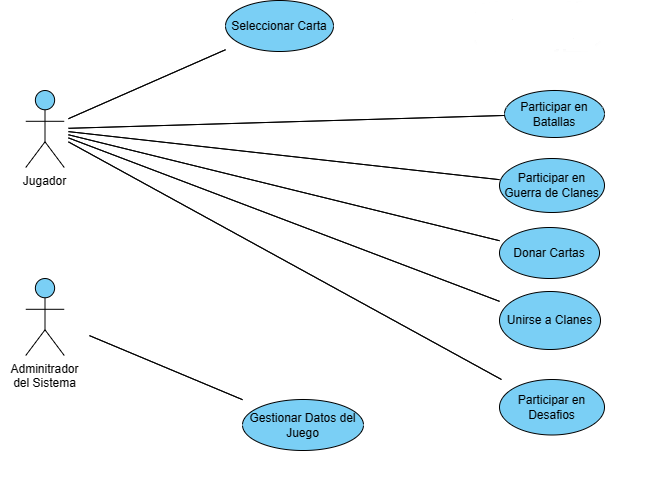
\includegraphics[width=0.5\textwidth]{../images/comic_use_cases.png}
\end{figure}

\begin{enumerate}
  \item Seleccionar Carta: Los jugadores pueden seleccionar cartas para usar en las batallas. Cada carta tiene habilidades y estadísticas únicas que pueden influir en el resultado de una batalla.
  \item Donar Carta: Los jugadores pueden donar cartas a otros miembros de su clan. Esto puede ayudar a los miembros del clan a mejorar sus mazos y avanzar en el juego.
  \item Unirse a Clanes: Los jugadores pueden unirse a clanes existentes o crear nuevos clanes. Dentro de un clan, los jugadores pueden colaborar, compartir cartas y participar en guerras de clanes juntos.
  \item Participar en Batallas: Los jugadores pueden participar en batallas uno a uno para ganar trofeos. El objetivo es destruir las torres del oponente mientras defienden las suyas.
  \item Participar en Desafíos: Los desafíos son eventos especiales donde los jugadores pueden ganar recompensas adicionales. Los jugadores deben acumular victorias en estos eventos para obtener las recompensas.
  \item Participar en Guerras de Clanes: Las guerras de clanes son eventos competitivos donde varios clanes compiten entre sí por trofeos y recompensas.
  \item Gestionar Datos del Juego: El administrador del sistema recopila y analiza datos sobre el comportamiento del juego para ayudar a diseñar nuevas formas de juego que atraigan a nuevos jugadores y mantengan a los actuales jugando.
\end{enumerate}

\begin{figure}[H]
  \centering
  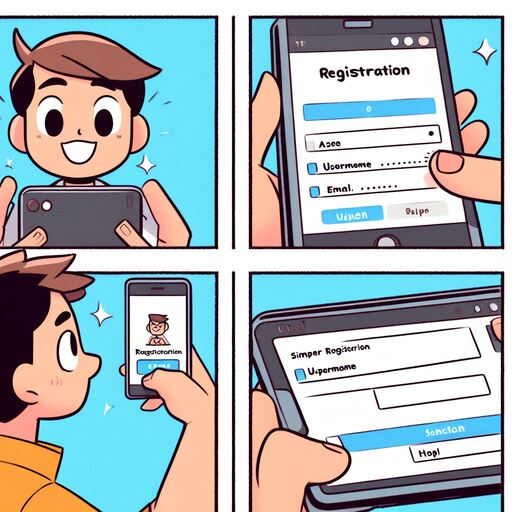
\includegraphics[width=0.8\textwidth]{../images/comic_registration.jpeg}
  \caption{Muestra a un  usuario registrándose en tu aplicación}
\end{figure}

\begin{figure}[H]
  \centering
  
\includegraphics[width=0.8\textwidth]{../images/comic_query_card_stats.jpeg}
  \caption{Muestra al usuario consultando las estadísticas de diferentes cartas}
\end{figure}

\begin{figure}[H]
  \centering
  
\includegraphics[width=0.8\textwidth]{../images/comic_query_clan_stats.jpeg}
  \caption{Muestra al usuario consultando las estadísticas de diferentes clanes}
\end{figure}

\begin{figure}[H]
  \centering
  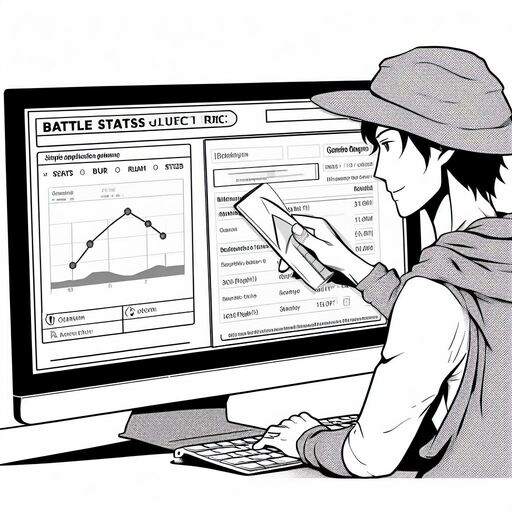
\includegraphics[width=0.8\textwidth]{../images/comic_query_match_stats.jpeg}
  \caption{Muestra al usuario consultando las estadísticas de diferentes batallas}
\end{figure}

\begin{figure}[H]
  \centering
  
\includegraphics[width=0.8\textwidth]{../images/comic_query_challenge_stats.jpeg}
  \caption{Muestra al usuario consultando las estadísticas de diferentes desafíos}
\end{figure}

\begin{figure}[H]
  \centering
  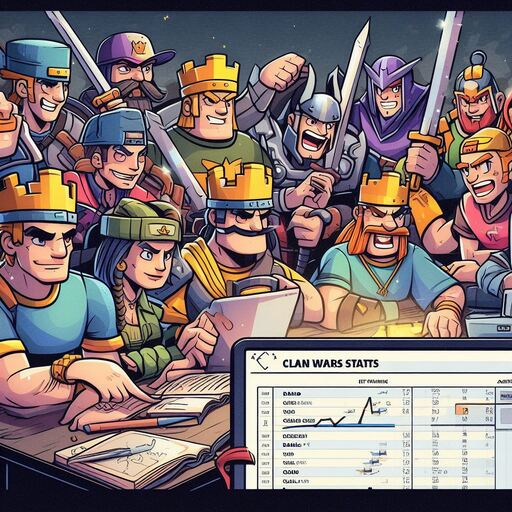
\includegraphics[width=0.8\textwidth]{../images/comic_query_clan_war_stats.jpeg}
  \caption{Muestra al usuario consultando las estadísticas de diferentes guerras de clanes}
\end{figure}

\begin{figure}[H]
  \centering
  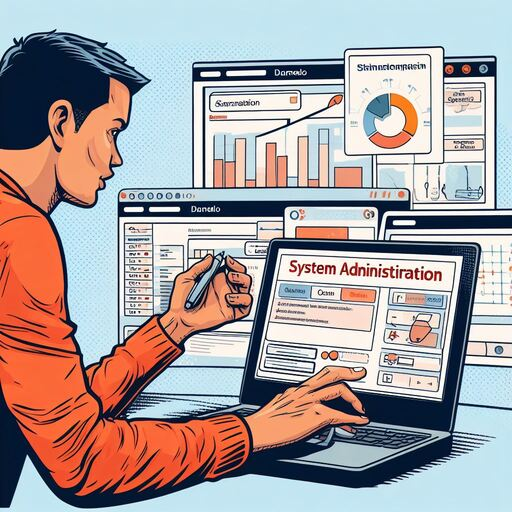
\includegraphics[width=0.8\textwidth]{../images/comic_administrator.jpeg}
  \caption{Muestra al administrador del sistema utilizando una interfaz administrativa para ver estadísticas del uso de la aplicación, ajustar la configuración y añadir nuevas características.}
\end{figure}

  % Copyright (c) 2023-2025
% This file is part of sep3cs.
%
% sep3cs is free software: you can redistribute it and/or modify
% it under the terms of the GNU General Public License as published by
% the Free Software Foundation, either version 3 of the License, or
% (at your option) any later version.
%
% sep3cs is distributed in the hope that it will be useful,
% but WITHOUT ANY WARRANTY; without even the implied warranty of
% MERCHANTABILITY or FITNESS FOR A PARTICULAR PURPOSE.  See the
% GNU General Public License for more details.
%
% You should have received a copy of the GNU General Public License
% along with sep3cs. If not, see <http://www.gnu.org/licenses/>.
%
\section{Enfoque Metodológico}

Dado que el proyecto que se desarrolla tiene un tiempo de desarrollo definido y unas especificaciones inmutables, la adopción de algunas de las metodologías de desarrollo de software ágiles en realidad solo aportaría una pequeña parte de los beneficios de dichas técnicas, mientras que sus desventajas no se atenuarían.

Por esto se decidió la adopción de una metodología híbrida que combina la planificación por adelantado de \textbf{RUP} con el desarrollo orientado a tests y el desarrollo en parejas de la programación extrema (\textbf{XP}). En concreto, lo que se pretende es un desarrollo iterativo horizontal típico de las técnicas ágiles usando test unitarios planeados de antemano para verificar cada iteración; al final de cada iteración, como el proyecto no plantea entregas periódicas de software (ni cambios en los requerimientos), simplemente se continuará con la siguiente.

Para concretar, la metodología adoptada tiene como características:

\begin{enumerate}
  \item[\(\cdot\)] Planificación previa de la fases de desarrollo y de las características que se añadirán al producto final.
  \item[\(\cdot\)] Construcción previa de tests unitarios usando para ello los casos de uso identificados durante el proceso de planificación.
  \item[\(\cdot\)] Desarrollo iterativo horizontal en la que cada iteración implementa una característica (posiblemente un caso de uso) dada.
  \item[\(\cdot\)] Revisión constante de código gracias a la implementación del desarrollo en parejas.
\end{enumerate}

  % Copyright (c) 2023-2025
% This file is part of sep3cs.
%
% sep3cs is free software: you can redistribute it and/or modify
% it under the terms of the GNU General Public License as published by
% the Free Software Foundation, either version 3 of the License, or
% (at your option) any later version.
%
% sep3cs is distributed in the hope that it will be useful,
% but WITHOUT ANY WARRANTY; without even the implied warranty of
% MERCHANTABILITY or FITNESS FOR A PARTICULAR PURPOSE.  See the
% GNU General Public License for more details.
%
% You should have received a copy of the GNU General Public License
% along with sep3cs. If not, see <http://www.gnu.org/licenses/>.
%
\section{Patrones de diseño y acceso a los datos}

Los patrones de datos que el software implementa son:

\begin{enumerate}
  \item[\(\cdot\)] \textit{Builder}: La familia de clases \lstinline|Data.Card|, \lstinline|Data.MagicCard|, \lstinline|Data.StructureCard| y \lstinline|Data.UnitCard| se construyen usando un este patron (mediante un objeto \lstinline|Utils.CardBuilder|).
  \item[\(\cdot\)] \textit{Singleton}: El objeto que representa la conexión con la base de datos (\lstinline|Data.Connection|) se trata de un singleton, de esta forma se optimiza su acceso dado que la aplicación es un servicio web y la creación de multiples conexiones por cada petición sería prohibitiva (aunque el \textbf{ORM} usado, \textit{Entity Framework}, implementa un sistema de \textit{caching} de las conexiones, es mejor manejarlo desde la aplicación que dejarlo en manos de un sistema genérico).
  \item[\(\cdot\)] \textit{Composition}: Los objetos que representan entidades en la base de datos (como \lstinline|Data.Card|) se componen en las instancias que representan relaciones (como \lstinline|Data.Match|), con lo que se asegura la representación de dichas relaciones.
\end{enumerate}

Los patrones de acceso a los datos que el software implementa son:

\begin{enumerate}
  \item[\(\cdot\)] \textit{Table Data Gateway}: El espacio de nombres (\textit{namespace}) \lstinline|Data| contiene clases que representan las tablas presentes en la base de datos (excepto \lstinline|Data.Connection| que representa la propia conexión con la base de datos). La clase \lstinline|Data.Connection| contiene colecciones de tipo \lstinline|System.Data.Entity.DbSet| que manejan el acceso a la base de datos, y usa patrones específicos del lenguaje para ofrecer acceso a esta (específicamente los métodos de las colecciones como \lstinline|OrderBy|, \lstinline|Add| y otros)
  \item[\(\cdot\)] \textit{Unit of Work}: Todos los cambios hechos en la clase \lstinline|Data.Connection| mediante los métodos descritos en el punto anterior se registran y luego se aplican a la base de datos subyacente mediante el método \lstinline|SaveChanges|. 
\end{enumerate}

  % Copyright (c) 2023-2025
% This file is part of sep3cs.
%
% sep3cs is free software: you can redistribute it and/or modify
% it under the terms of the GNU General Public License as published by
% the Free Software Foundation, either version 3 of the License, or
% (at your option) any later version.
%
% sep3cs is distributed in the hope that it will be useful,
% but WITHOUT ANY WARRANTY; without even the implied warranty of
% MERCHANTABILITY or FITNESS FOR A PARTICULAR PURPOSE.  See the
% GNU General Public License for more details.
%
% You should have received a copy of the GNU General Public License
% along with sep3cs. If not, see <http://www.gnu.org/licenses/>.
%
\section{Modelo Conceptual (MERX) de la base de datos}

\subsection*{Administrador}
\begin{figure}[H]
\centering
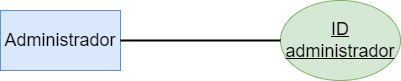
\includegraphics[width=0.5\textwidth]{../images/merx_administrator.png}
\caption{Administrador}
\end{figure}

\subsection*{Carta}
\begin{figure}[H]
\centering
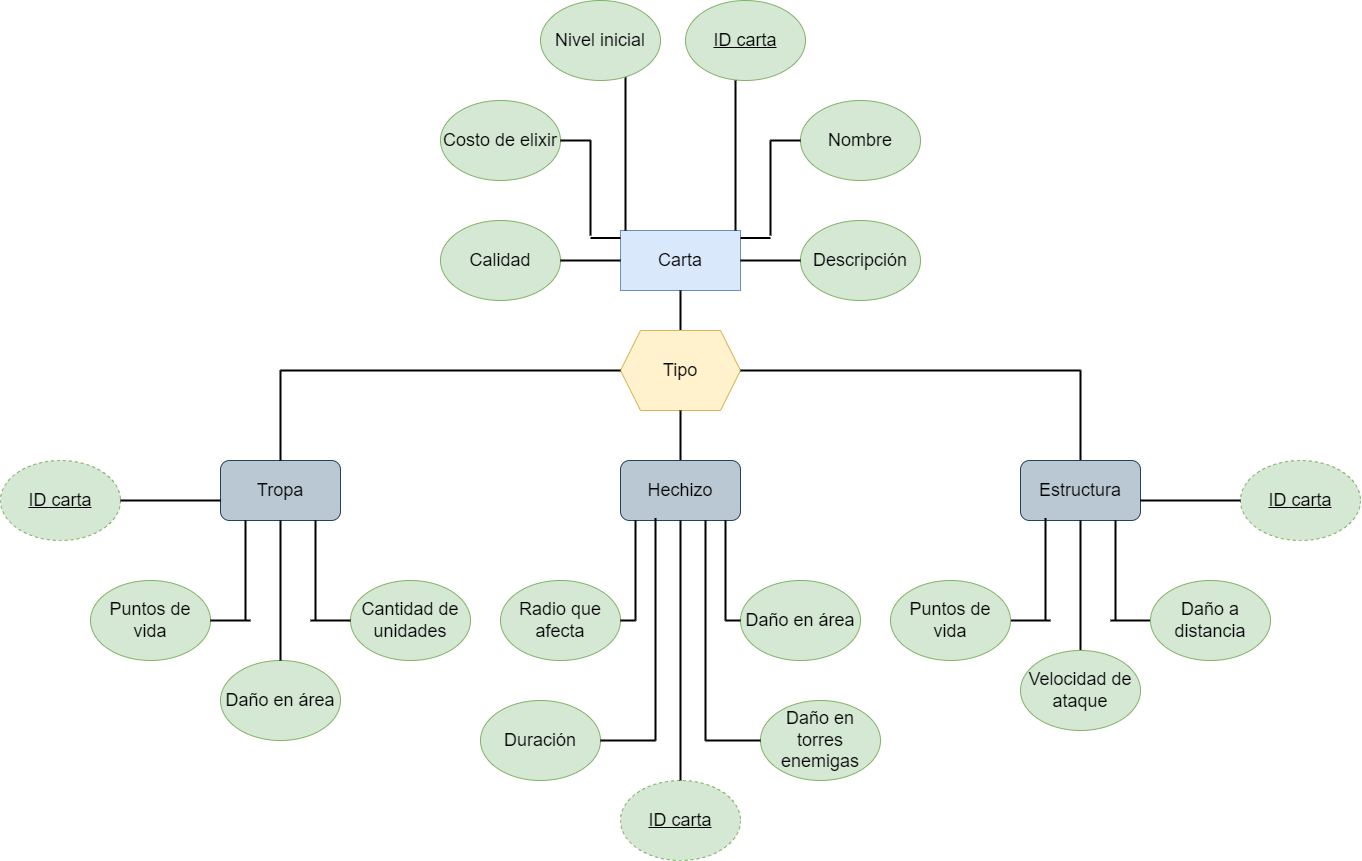
\includegraphics[width=0.98\textwidth]{../images/merx_card.png}
\caption{Carta}
\end{figure}

\subsection*{Jugador}
\begin{figure}[H]
\centering
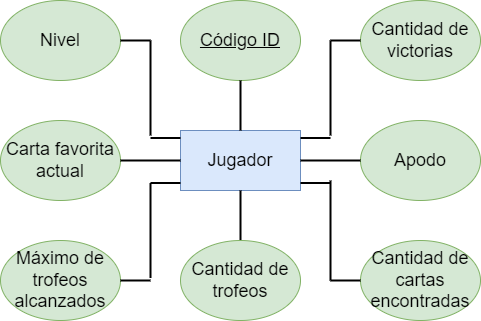
\includegraphics[width=0.5\textwidth]{../images/merx_player.png}
\caption{Jugador}
\end{figure}

\subsection*{Partida}
\begin{figure}[H]
\centering
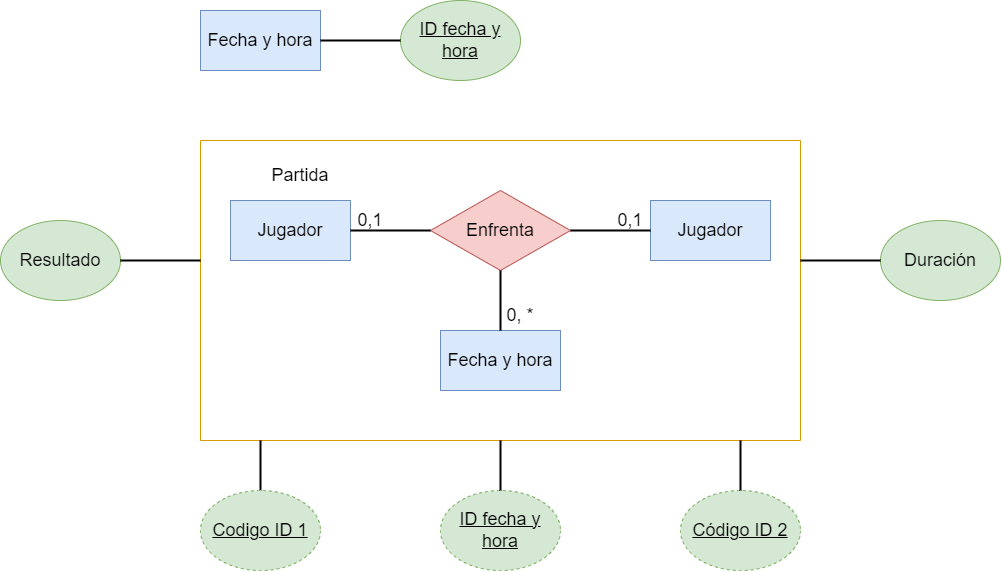
\includegraphics[width=0.80\textwidth]{../images/merx_match.png}
\caption{Partida}
\end{figure}

\subsection*{Carta de Jugador}
\begin{figure}[H]
\centering
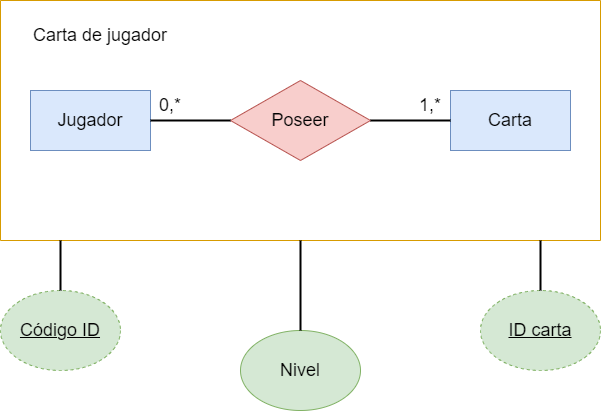
\includegraphics[width=0.60\textwidth]{../images/merx_playercard.png}
\caption{Carta de Jugador}
\end{figure}

\subsection*{Clan}
\begin{figure}[H]
\centering
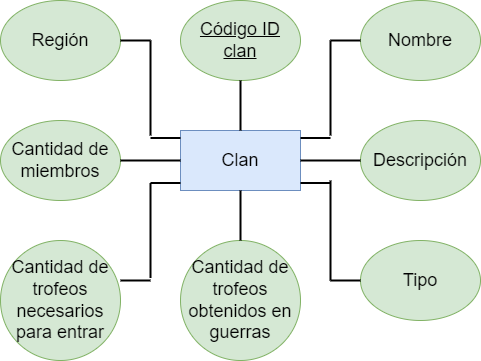
\includegraphics[width=0.60\textwidth]{../images/merx_clan.png}
\caption{Clan}
\end{figure}

\subsection*{Jugador Clan}
\begin{figure}[H]
\centering
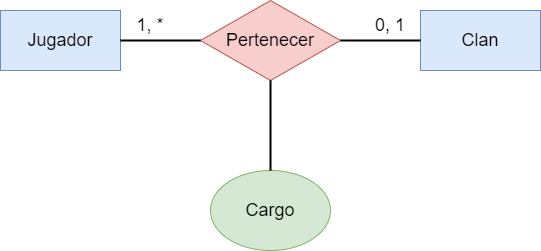
\includegraphics[width=0.5\textwidth]{../images/merx_playerclan.png}
\caption{Jugador Clan}
\end{figure}

\subsection*{Desafío}
\begin{figure}[H]
\centering
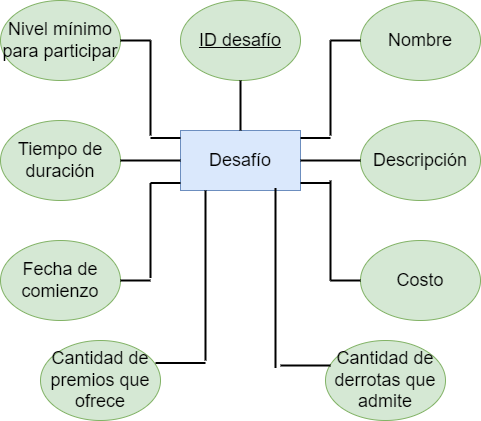
\includegraphics[width=0.5\textwidth]{../images/merx_challenge.png}
\caption{Desafío}
\end{figure}

\subsection*{Donación}
\begin{figure}[H]
\centering
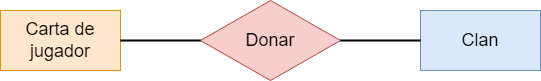
\includegraphics[width=0.5\textwidth]{../images/merx_gift.png}
\caption{Donación}
\end{figure}

\subsection*{Guerra}
\begin{figure}[H]
\centering
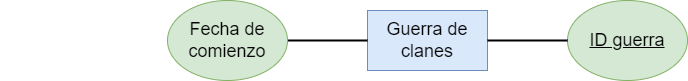
\includegraphics[width=0.5\textwidth]{../images/merx_war.png}
\caption{Guerra}
\end{figure}

\subsection*{Jugador Desafío}
\begin{figure}[H]
\centering
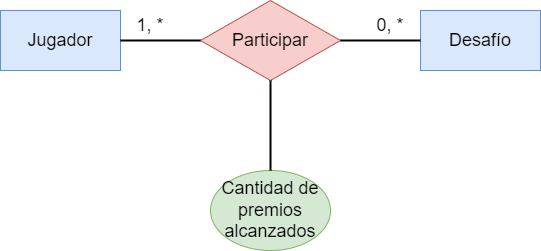
\includegraphics[width=0.5\textwidth]{../images/merx_playerchallenge.png}
\caption{Jugador Desafío}
\end{figure}

\subsection*{Relación Guerra }
\begin{figure}[H]
\centering
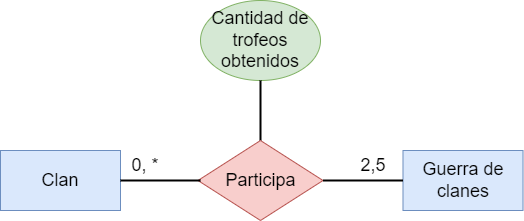
\includegraphics[width=0.5\textwidth]{../images/merx_clanwar.png}
\caption{Relación Guerra}
\end{figure}

\end{document}
